\documentclass[a4paper, 12pt]{article}

\usepackage[ngerman]{babel}
\usepackage[utf8]{inputenc}
\usepackage[T1]{fontenc}

\usepackage{fancyhdr}

\lhead[]{DHBW Karlsruhe}
\chead[]{}
\rhead[]{22. Oktober 2018}

\lfoot[]{Daniel Schädler \& Jean-Pierre Hotz}
\cfoot[]{}
\rfoot[]{\thepage}

\usepackage[pagesize]{typearea}

\usepackage[a4paper,headheight=62pt,margin=2.5cm,includeheadfoot]{geometry}
 
\usepackage{textcomp}

\usepackage{float}
\usepackage{graphicx}
\usepackage{wrapfig}

\usepackage{caption}
\usepackage{subcaption}

\usepackage{setspace}
\onehalfspacing

\usepackage{enumitem}

%Preamble
\usepackage{listings}
\usepackage{color}

\pagestyle{empty}

%\definecolor{name}{rgb}{0.5,0.5,0.5}
%\lstset{key1=value1,key2=value2} % Define listings style
 
%Document body
%\begin{lstlisting}
% Add code here
%\end{lstlisting}
 
% Or load from file
%\lstinputlisting{filename.java}

\definecolor{sourcecodered}{rgb}{0.6,0,0} % for strings
\definecolor{sourcecodegreen}{rgb}{0.25,0.5,0.35} % comments
\definecolor{sourcecodepurple}{rgb}{0.5,0,0.35} % keywords
\definecolor{sourcecodedocblue}{rgb}{0.25,0.35,0.75} % javadoc
 
\lstset{
	language=C,                                    % the language of the code
	basicstyle=\ttfamily\small,                    % the size of the fonts that are used for the code
	keywordstyle=\ttfamily\small,                  % keyword style
	stringstyle=\ttfamily\small,                   % string literal style
	commentstyle=\ttfamily\small,                  % comment style
	numbers=none,                                  % where to put the line-numbers; possible values are (none, left, right)
	numberstyle=\small\color{black},               % the style that is used for the line-numbers
	numbersep=6pt,                                 % how far the line-numbers are from the code
	tabsize=4,	                   	               % sets default tabsize to 4 spaces
	showspaces=false,                              % show spaces everywhere adding particular underscores; it overrides 'showstringspaces'
	showstringspaces=false,                        % underline spaces within strings only
	showtabs=false,                                % show tabs within strings adding particular underscores
%	title=\lstname,                                % show the filename of files included with \lstinputlisting; also try caption instead of title
	breaklines=true,                               % sets automatic line breaking
	breakatwhitespace=true,                             % sets if automatic breaks should only happen at whitespace
	frame=single,	                                     % adds a frame around the code
	rulecolor=\color{black},                             % if not set, the frame-color may be changed on line-breaks within not-black text (e.g. comments (green here))
	literate=%
		{Ö}{{\"O}}1
		{Ä}{{\"A}}1
		{Ü}{{\"U}}1
		{ß}{{\ss}}1
		{ü}{{\"u}}1
		{ä}{{\"a}}1
		{ö}{{\"o}}1
		{~}{{\textasciitilde}}1
	% backgroundcolor=\color{white},      % choose the background color; you must add \usepackage{color} or \usepackage{xcolor}; should come as last argument
	% captionpos=b,                       % sets the caption-position to bottom
	% deletekeywords={...},               % if you want to delete keywords from the given language
	% escapeinside={\%*}{*)},             % if you want to add LaTeX within your code
	% extendedchars=true,                 % lets you use non-ASCII characters; for 8-bits encodings only, does not work with UTF-8
	% keepspaces=true,                    % keeps spaces in text, useful for keeping indentation of code (possibly needs columns=flexible)
	% morekeywords={*,...},               % if you want to add more keywords to the set
	% stepnumber=2,                       % the step between two line-numbers. If it's 1, each line will be numbered
}

\usepackage{amssymb}
\usepackage{amsmath}

\usepackage{braket}

\usepackage{tikz}

\usetikzlibrary{arrows,decorations.markings}

\tikzstyle{arrow} = [->,>=stealth]
\tikzset{nicearrow/.style={decoration={markings,mark=at position 1 with %
			{\arrow[scale=3,>=stealth]{>}}},postaction={decorate}}}

\usepackage{acronym}

\usepackage[font=footnotesize]{caption}

\usepackage{tcolorbox}

\begin{document}
	
	
	\begin{center}
		\newcommand{\HRule}{\rule{\linewidth}{0.5mm}}
		\HRule \\[0.8cm]
		{ \huge \bfseries Git \& GitHub Tutorial}\\[0.4cm]
		{\LARGE \bfseries Software-Engineering}\\[0.4cm]
		\HRule \\[1.5cm]
		\begin{center}
			by\\[0.2cm]
			Daniel Schädler and Jean-Pierre Hotz\\[0.7cm]
			22. October 2018
		\end{center}
		\vfill
		Course: TINF17B4\\
		Lecturer: K. Berkling, Ph.D.
	\end{center}
	\newpage
	\pagestyle{fancy}

	\section*{Disclaimer}
		
		Since the usage of the git commandline and ui-clients for git work in basically the same way this (written) tutorial only shows you how to use Git and GitHub from the commandline. Other UIs will be shown during the presentation, though.
		
		On the topic of commandlines: Every command / file shown in this tutorial is enclosed in a box with a black outline. In case a command is shown, any user input will be denoted by a preceding dollar sign (as it's done by Git for Windows).

	\section{Jean-Pierre}
		
	\section{Use your Github user in Git}
	
		To use your GitHub user in Git (and thus also link your local commits to your Github account) you can change the user name and e-mail-adress as follows:
		
		\begin{lstlisting}
$ git config --global user.name "<your Github-Username>"
$ git config --global user.email <your Github-E-Mail>
		\end{lstlisting}
		
		In case you need verification Git will ask you for valid credentials.
				
	\section{Make Git ignore certain files / folders}
		
		To make Git ignore certain files and folders you'll have to create an \lstinline|.gitignore|-file. Every line in this file will represent a pattern to excluded files, also called a rule. In case you want files with a certain pattern to be only excluded in the root-directory you'll have to precede the pattern with a forward-slash \lstinline|'/'|. To exclude folders you'll have to follow the pattern by a forward-slash \lstinline|'/'|. To make a pattern match anything you can simply type an asterisk \lstinline|'*'|. To create an exception to a general rule, you can simply give a more specific rule (for the files you want to \textbf{include}), and precede that rule with a bang \lstinline|'!'|.
		
		The \lstinline|.gitignore|-file is always useful to exclude IDE-specific files (e.g. \lstinline|.iml|-files in IntelliJ) or compiled binaries. An example \lstinline|.gitignore|-file for a personal Java-project is shown below:
		
		\begin{lstlisting}
*.iml
target/
.idea/
!.idea/copyright/
lib/
		\end{lstlisting}

	\section{Creation of a local repository}

		There are two different ways to create a local repository, which is used to track your own changes in the exisiting code.

		The first option you have is to create an \glqq empty\grqq~ repository. In case this is done in a folder, which contains files, these files are not being tracked yet. This can be done using the following command.

		\begin{lstlisting}
$ git init
		\end{lstlisting}

		The second option (which is probably used more often in teamwork), is to clone from an already existing remote repository, like an repository on GitHub or, an ordinary Git repository, you or a team member has created on a simple file server.

		\begin{lstlisting}
$ git clone https://github.com/<User-Name>/<Repository-Name>.git
		\end{lstlisting}

	\section{Make versions of files}
	
		Since Git and Github is all about file versioning, we can make Git capture single versions of files with commits. Before creating commits though, we'll have to add changes that are to be included in the version we want to capture. This process is called 'staging changes' and can be done either by staging all changes, or by only staging certain files.
		
		\begin{lstlisting}
> git add --all
> git add <files>
		\end{lstlisting}
		
		To then create a commit with the staged changes you can use following command:
		
		\begin{lstlisting}
> git commit -m "<Commit-message (can be multi-line)>"
		\end{lstlisting}
		
		Commit-messages are not easy to get right, especially as a beginner to Git, but good commit messages make your work with Git much easier. Especially since this allows you to review your commit history efficiently and see who changed what, and why they did so. To explain commit messages we'll have to break it down to its components. A commit message always has a caption, which is usually the first line of the actual message. This caption should be \textbf{separated} from the body of the message \textbf{by a blank line}. Also the caption should always be \textbf{capitalized}, and have a \textbf{maximum of 50 characters} in it. A caption is supposed to make sense to be filled into the sentence \glqq If applied, this commit will \_\grqq, which means that the imperative mood is to be used.The body of the commit message should be wrapped at \textbf{72 characters}, and should explain what has been done and why this has been done. You sould omit how you achieved what you have done, since this (should be) easily readable from the changes you have made. \footnote{This paragraph heavily relies on the blog posts found at \lstinline|https://medium.com/@nawarpianist/git-commit-best-practices-dab8d722de99| and \lstinline|https://chris.beams.io/posts/git-commit/|}
		
	\section{Showing changes and commits}
		
		There are different ways of showing your changes and commits. To show the differences between two commits or the current changes to certain or all files you can simply use \lstinline|diff|.
		
		\begin{lstlisting}
> git diff <commit1> <commit2>
> git diff <commit> <filesToCompare>
> git diff
		\end{lstlisting}
		
		The first command will list every change you have made between the given commits. The second will list every change you have made in the given files since the given commit, and the last command will list every change you have made since the last commit. Also note that there are more options on how to use this command than we show you here.
		\newpage
		
		To show files which have been changed, created, deleted or moved (while the last two options only apply to tracked files) you can use the \lstinline|status|-command. It also shows which files are not tracked, or which changes are currently staged to be committed.
		
		\begin{lstlisting}
> git status
		\end{lstlisting}
		
		To show the commit history you can use the \lstinline|log|-command. To look at the commit history makes sense, whenever you need to determine the hashes of certain commits (can be used e.g. for \lstinline|diff|) or to see whether something has already been done by someone.
		
		\begin{lstlisting}
> git log
		\end{lstlisting}
		
	\section{Managing a remote repository}
	
		To manage a remote repository (like a repository hosted on Github) you'll have to know two basic commands. Those are push your commits (i.e. versions) to the remote repository, or pull all the commits from the repository. And those are also the names of the git-commands.
		
		\begin{lstlisting}
> git push
> git pull
		\end{lstlisting}
		
		In case you have created an empty repository, you'll have to add the remote repository first, though. This can be done with the \lstinline|remote-add|-command. The name of a remote repository usually is \lstinline|origin|.
		
		\begin{lstlisting}
> git remote add <Name> <URL>
		\end{lstlisting}
		
		To then push you'll also have to set this repository as the repository to push to.
		
		\begin{lstlisting}
> git push -u <Name> <Branch>
		\end{lstlisting}
		
		After this your pushes on the given branch will automatically pushed to the given remote repository.

	\section{Marking important points in your history}
	
		Git allows you to \lstinline|tag| specific points in your history, which is usually used to mark specific release versions. Those tags can be listed with the \lstinline|--list| option.
		
		\begin{lstlisting}
> git tag --list
		\end{lstlisting}
		
		To create a tag with a specific message you can use the options \lstinline|-a| and \lstinline|-m|. specific release versions. In case you want to create a tag after a certain commit you can simply state this commits hash (or the beginning of it until it is unique) after the command.
		
		\begin{lstlisting}
> git tag -a <your version> -m "<your message>" <hash of the commit>
		\end{lstlisting}
		
		To share tags to remote repositories (which is not done automatically) you'll either push a single tag with the following command: 
		
		\begin{lstlisting}
> git push origin <your version>
		\end{lstlisting}
		
		Or to push all tags that have not yet been pushed, you can use this command:
		
		\begin{lstlisting}
> git push origin --tags
		\end{lstlisting}
		\newpage
		
	\section{Daniel}
			
	\section{branches}
	
		Git is not only useful for working alone. It is used to manage many users working in a single project on different branches. Branches are different directions the project is heading of to. These can be represented by just older or more recent code or different features that are developed at the same time. To simplify working with different half implemented features, git uses branches. A user that creates a commit on a given branch, lets call it branch A, does not affect work that is already or concurrently done on Branch B. Therefore these two branches are seperate from each other. They may come back together at some point, but they can also stay divergent all the time. Normally the use case of git is to have a master branch of the released version of the product with a develop branch that has experimental new features. Then there are different feature branches that all implement a single new feature. These branches are where the developers spent most of their time. They implement the features they want to and then merge the branch back into develop where the code waits to get released with the next version.
		
		\begin{figure}[h]
			\centering
			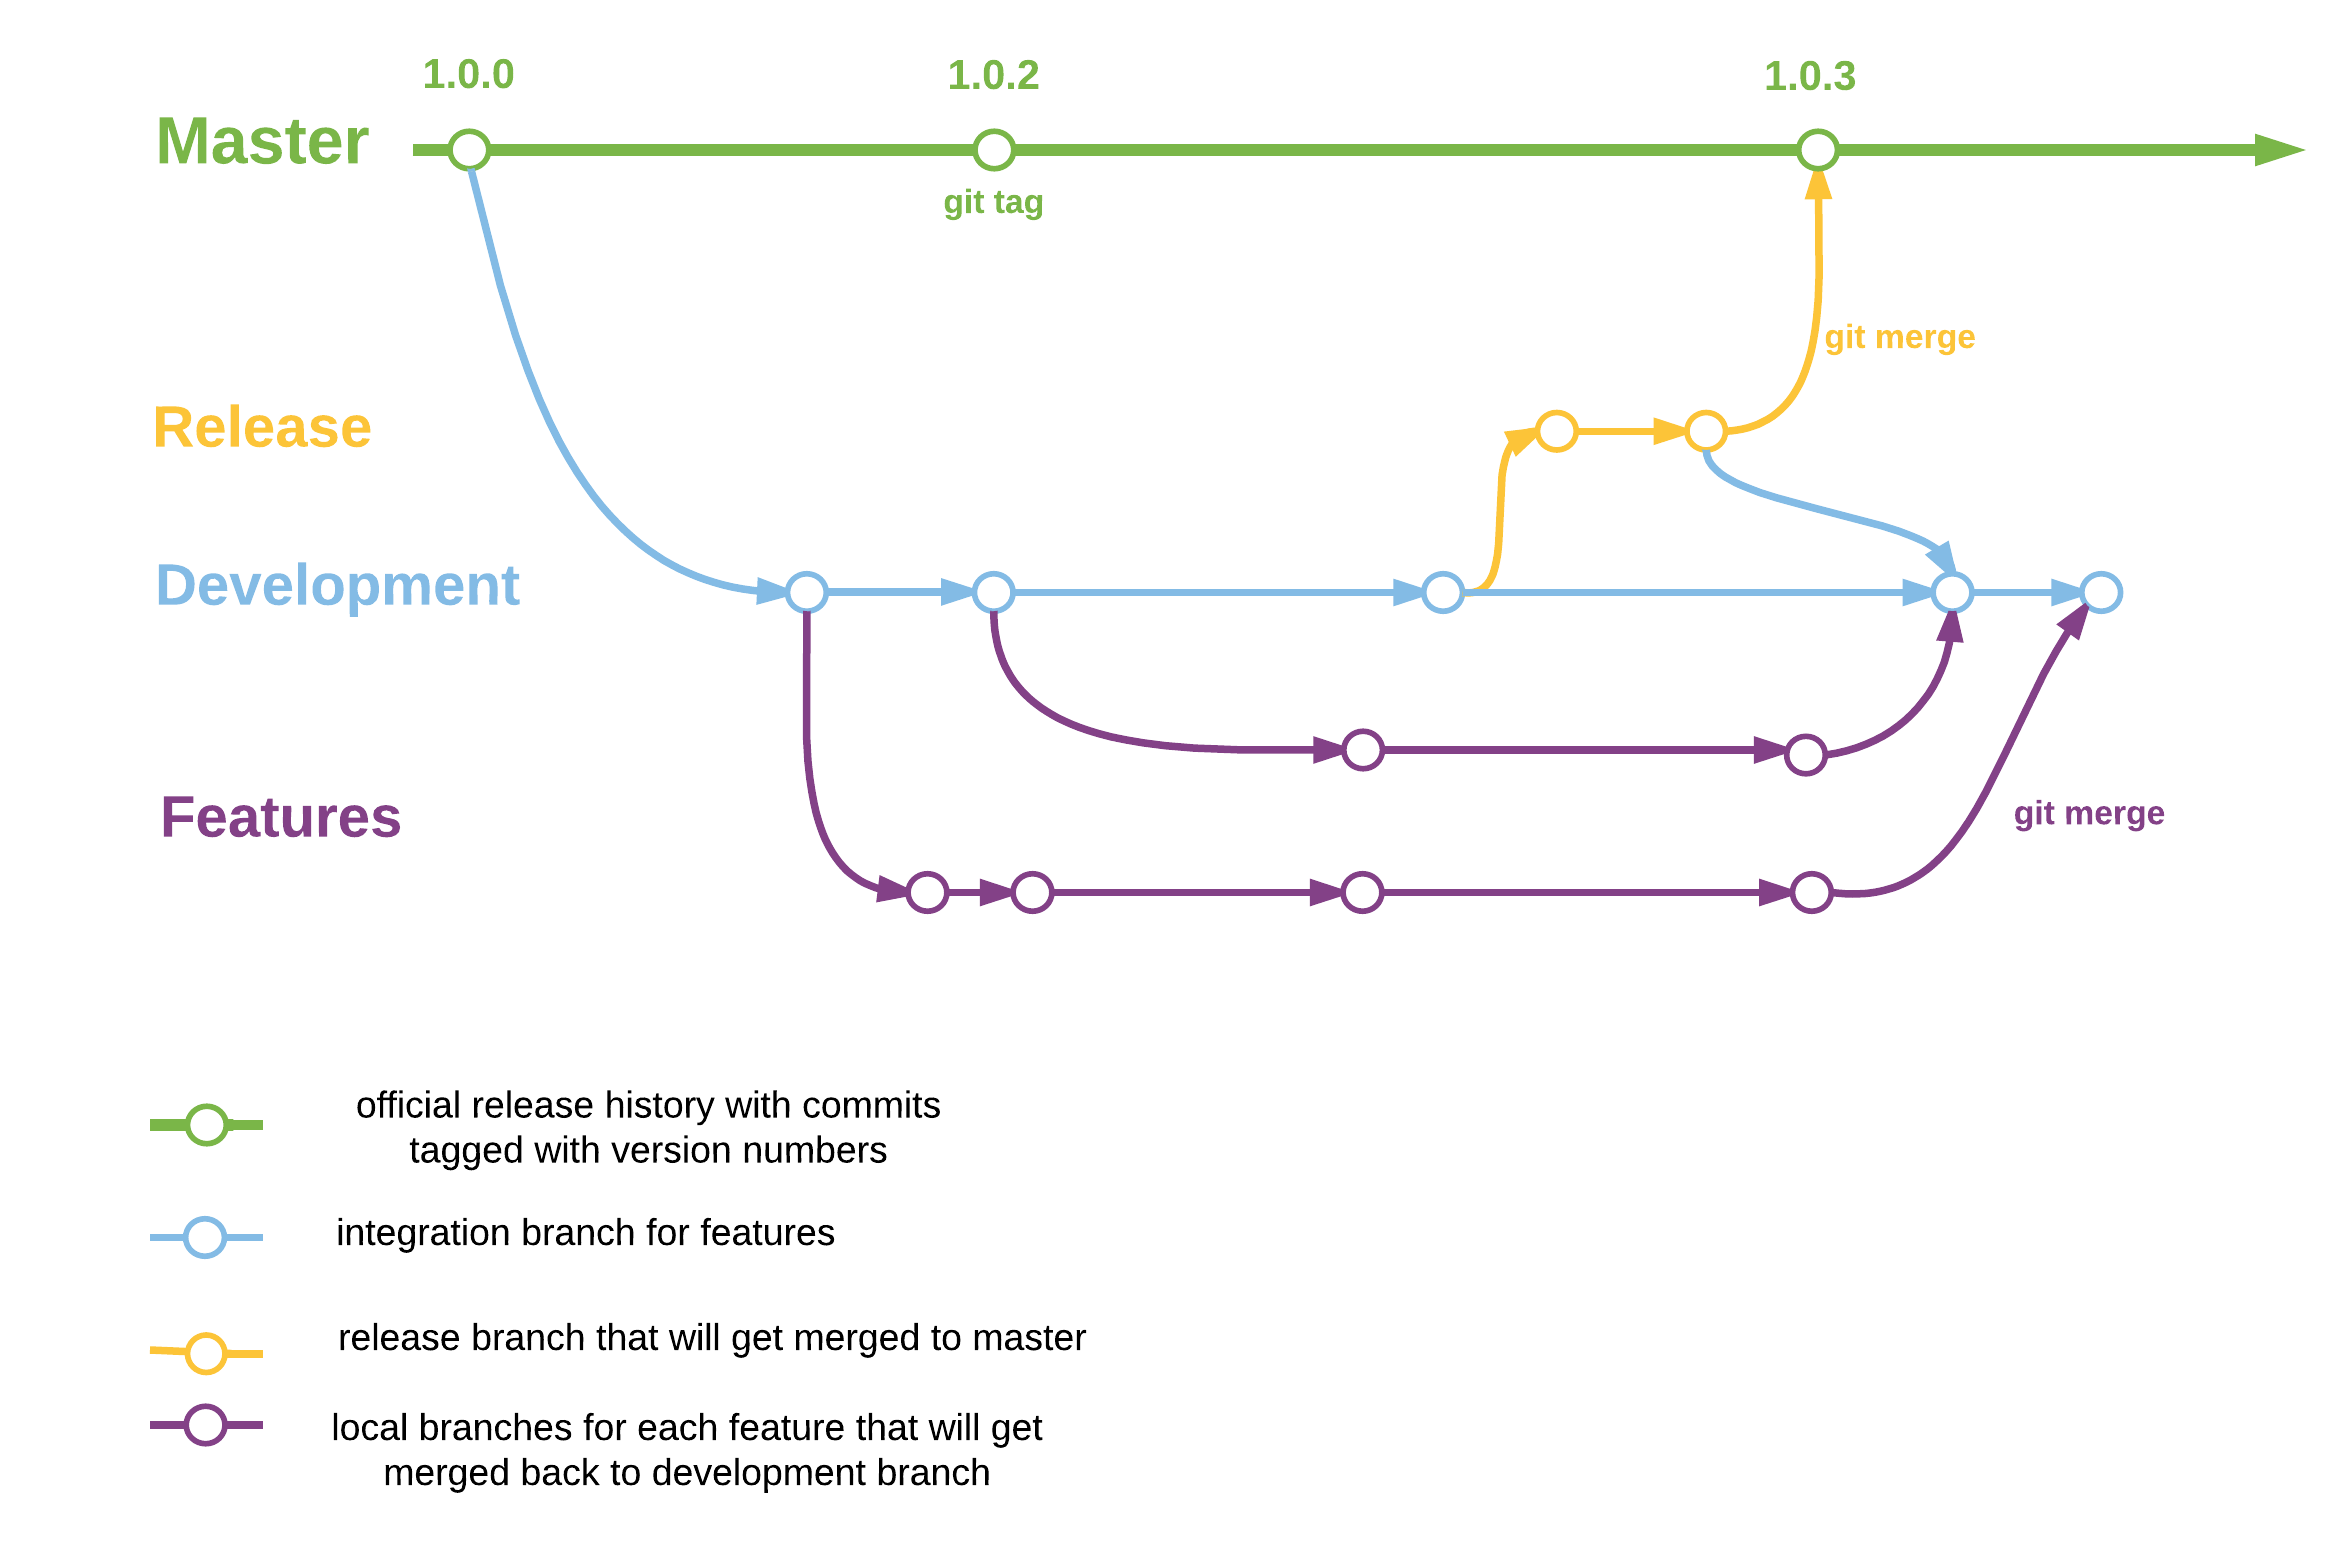
\includegraphics[width=.725\linewidth]{gitbranches.png}
			\label{fig1}
			\caption{Here you can see the mentioned workflow. Source: https://help.talend.com/reader/GDDhoNyPTrERkrITzE6qPQ/QhAXF8ijSOHq~lhrVCoLKQ}
		\end{figure}
		
	\section{merging}
		
		To bring two branches back together the user has to merge them. This can either be done by a merge commit or by rebasing the branch that needs to be merged onto the branch it needs to be merged into. A merge commit is a commit, that merges the two branches. The merge itself is started by:
		
		\begin{lstlisting}
> git merge <branchname>
		\end{lstlisting}
		
		This merges the given branch into the current branch. When there are no conflicting changes, meaning no conflicting lines, the merge commit is empty and the branches are merged easily. When there are conflicting changes, these changes pause the merge process and need to be resolved before continuing. The conflicting lines then get marked in the File and the user has to decide, which version is right. After doing so, the merge is continues by typing 
		
		\begin{lstlisting}
> git merge --continue
		\end{lstlisting}
		
	\section{rebasing}
		When you want to avoid a merge commit, a rebase is what you want. Rebasing a branch means to change the point, where it is diverging from the other branches to the point given in the command.
		
		\begin{figure}[h]
			\centering
			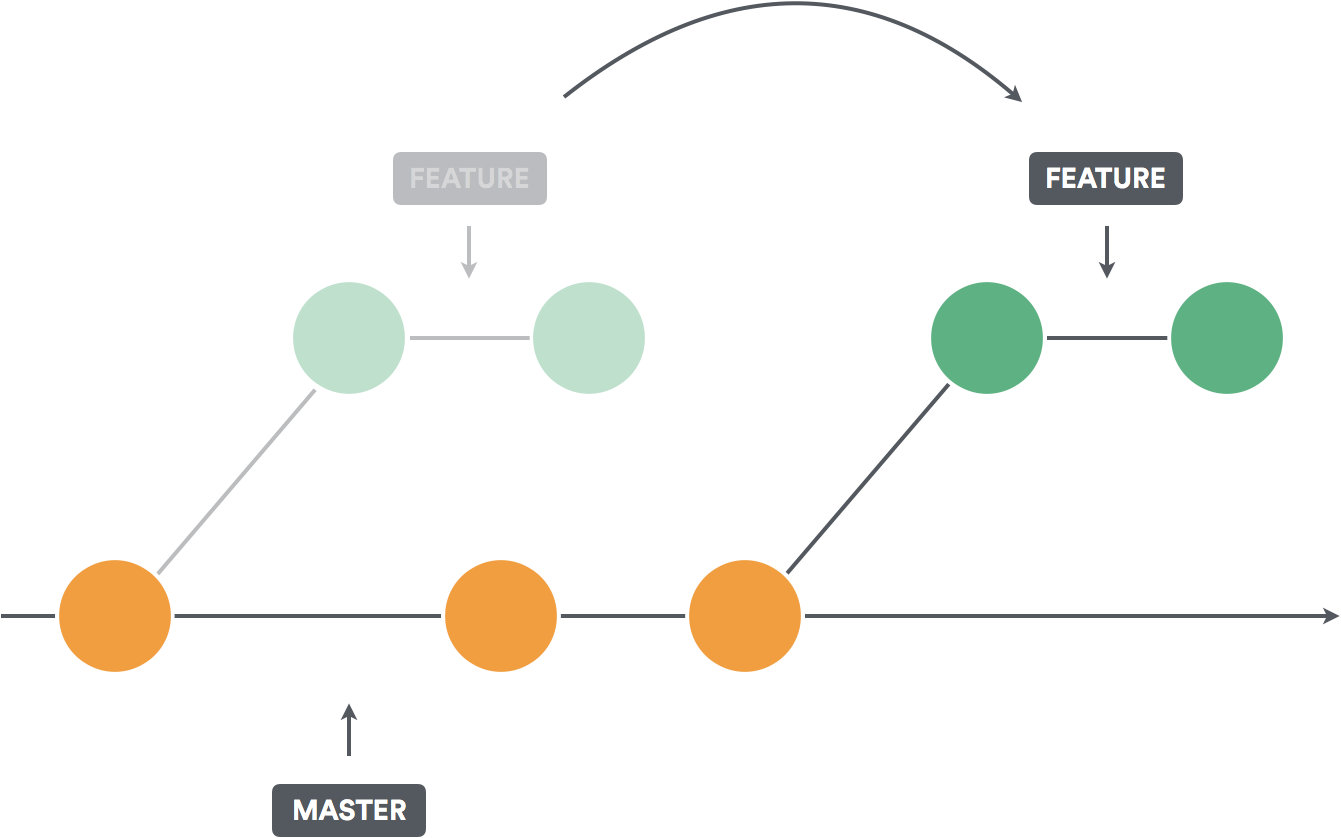
\includegraphics[width=.725\linewidth]{gitrebase.png}
			\label{fig1}
			\caption{Here you can see the mentioned workflow. Source: https://help.talend.com/reader/GDDhoNyPTrERkrITzE6qPQ/QhAXF8ijSOHq~lhrVCoLKQ}
		\end{figure}
		
		\begin{lstlisting}
> git rebase <commit id / branch>
		\end{lstlisting}
		
		When typing this, git rolls back to the point where the two branches diverged, then applies all the commits that happened to the point you specified in your command and then tries to apply all the commits that happened on the current branch since it diverged. Again, if there are no conflicting changes, the rebase is successful and your branch can now be merged with the \lstinline|--ff-only| option, meaning all the changes will be copied over to the branch you are merging into without creating new commits.
		
	\section{remotes}
		
		Working locally with git is fine and good, but when you want to efficiently share your work you will need a remote. There are many services that serve as a git remote like GitHub, Bitbucket or Gitlab. These remotes just serve as a online copy of the local git tracked directory. This has the advantage, that you do not need internet access all the time to work with other people. You always have the full history of the git directory on your computer.
		
	\section{GitHub}
		
		As we are using GitHub in our group, we focus on GitHub for now. But most of the features mentioned here work pretty much the same for the other services. The first thing is 
		
		\subsubsection{branch protection}
		
			As you work with other people, it gets more and more important to secure some branches. These secured branches can (depending on the configuration) normally not be simply pushed to. Also you can just disable force pushes, making the commits immutable.
		
		\subsubsection{pull requests}
		
			If a branch is protected from pushing, you will probably need a pull request for your changes to be added to it. A pull request, is a request you make for the other collaborators to check your changes and review them. Once you reach the configured threshold of reviews, your changes can be merged. Within the GUI you then have the same merge options as previously explained.
		
		\subsubsection{issues}
		
			On GitHub there is also a Ticket System for users that have problems with your project. One can raise a bug or create a ticket in general to which the collaborators can write comments and do their best to resolve the issue.

\end{document}